\documentclass[dvipdfmx,uplatex,12pt]{jsarticle}

\usepackage{amssymb}
\usepackage{tikz,pgf}
\usepackage{listings}
\usepackage{color}
\definecolor{lightgray}{rgb}{.9,.9,.9}
\definecolor{darkgray}{rgb}{.4,.4,.4}
\definecolor{purple}{rgb}{0.65, 0.12, 0.82}

\lstdefinelanguage{JavaScript}{
  keywords={typeof, new, true, false, catch, function, return, null, catch, switch, var, if, in, while, do, else, case, break, let},
  keywordstyle=\color{blue}\bfseries,
  ndkeywords={class, export, boolean, throw, implements, import, this},
  ndkeywordstyle=\color{darkgray}\bfseries,
  identifierstyle=\color{black},
  sensitive=false,
  comment=[l]{//},
  morecomment=[s]{/*}{*/},
  commentstyle=\color{purple}\ttfamily,
  stringstyle=\color{red}\ttfamily,
}

\lstset{
   language=JavaScript,
   backgroundcolor=\color{lightgray},
   extendedchars=true,
   basicstyle=\footnotesize\ttfamily,
   showstringspaces=false,
   showspaces=false,
   numbers=left,
   numberstyle=\footnotesize,
   numbersep=9pt,
   tabsize=2,
   breaklines=true,
   showtabs=false,
   captionpos=b
}





\begin{document}

ペンローズタイル張りを描く基本的なアルゴリズムは
以下のような感じです。
まず、ペンローズタイル張りにとって基本的な定数である
{\em 黄金比}を
\[
 \varphi = \frac{1+\sqrt{5}}{2}
\]
と定めます。黄金比が満たす基本的関係式
\[
 \varphi^2 = \varphi + 1
\]
とその変形
\[
 \frac{1}{\varphi} = \varphi-1
\]
はこの後特に重要な働きをします。

\begin{tikzpicture}[scale=3]
 \node [inner sep=0pt,minimum size = 0pt] (A)at (0,0){};
 \node [inner sep=0pt,minimum size = 0pt] (B)at (1,0){};
 \node [inner sep=0pt,minimum size = 0pt] (C)at (36:1){};
 \draw[->,>=latex] (A) edge (B);
 \draw[->,>=latex] (B) edge (C);
 \draw[->,>=latex] (C) edge (A);
 \draw (A) node[below] {$0 = (0,0,0,0,0)$};
 \draw (B) node[below] {$1 = (1,0,0,0,0)$};
 \draw (C) node[above] {$\zeta = (0,1,0,0,0)$};

 \draw (1.65,0.3) node[above]{$\varphi$倍拡大};
 \draw[->,>=latex,line width=3] (1.5,0.3) -- (1.8,0.3);

 \begin{scope}[xshift=2cm,scale=1.61803]
 \node [inner sep=0pt] (A1)at (0,0){};
 \node [inner sep=0pt] (B1)at (1,0){};
 \node [inner sep=0pt] (C1)at (36:1){};
 \draw[->,>=latex] (A1) edge (B1);
 \draw[->,>=latex] (B1) edge (C1);
 \draw[->,>=latex] (C1) edge (A1);
 \draw (A1) node[below] {$0 = (0,0,0,0,0)$};
 \draw (B1) node[below] {$\varphi = (0,1,0,0,-1)$};
 \draw (C1) node[above] {$\varphi\zeta = ({\color{red}\bf 1},0,1,0,0)$};
 \end{scope}

 \draw[->,>=latex,line width=3] (2.3,-0.6) -- (2.1,-0.8);
 \draw (2.2,-0.7) node [right] {細分};

 \begin{scope}[yshift=-1.5cm,scale=1.61803]
 \node [inner sep=0pt] (A1)at (0,0){};
 \node [inner sep=0pt] (B1)at (1,0){};
 \node [inner sep=0pt] (C1)at (36:1){};
 \node [inner sep=0pt] (D1)at (.61803,0){};
 \draw[>=latex] (A1) edge (D1);
  \draw[>=latex] (D1) edge (C1);
 \draw[>=latex] (C1) edge (A1);
  \draw[>=latex] (C1) edge (D1);
  \draw[>=latex] (D1) edge (B1);
  \draw[>=latex] (B1) edge (C1);
 \draw (D1) node[below] {$\varphi:1 内分点 1 = (1,0,0,0,0)$};
  \draw[->,>=stealth,line width=0.5,blue] (18:0.6) arc (18:(18-360):0.1);
  \draw[->,>=stealth,line width=0.5] (10:0.9) arc (18:(18+360):0.065);
 \end{scope}

\end{tikzpicture}

\vspace{3cm}

\begin{tikzpicture}[scale=3]
 \node [inner sep=0pt,minimum size = 0pt] (A)at (0,0){};
 \node [inner sep=0pt,minimum size = 0pt] (B)at (1,0){};
 \node [inner sep=0pt,minimum size = 0pt] (C)at (36:1.61803){};
 \draw[->,>=latex] (A) edge (B);
 \draw[->,>=latex] (B) edge (C);
 \draw[->,>=latex] (C) edge (A);
 \draw (A) node[below] {$0 = (0,0,0,0,0)$};
 \draw (B) node[below] {$1 = (1,0,0,0,0)$};
 \draw (C) node[above] {$\varphi\zeta = (-1,0,1,0,0)$};

 \draw (1.65,0.3) node[above]{拡大};
 \draw[->,>=latex,line width=3] (1.5,0.3) -- (1.8,0.3);

 \begin{scope}[xshift=2cm,scale=1.61803]
 \node [inner sep=0pt] (A1)at (0,0){};
 \node [inner sep=0pt] (B1)at (1,0){};
 \node [inner sep=0pt,minimum size = 0pt] (C1)at (36:1.61803){};
 \draw[->,>=latex] (A1) edge (B1);
 \draw[->,>=latex] (B1) edge (C1);
 \draw[->,>=latex] (C1) edge (A1);
 \draw (A1) node[below] {$0 = (0,0,0,0,0)$};
 \draw (B1) node[below] {$1 = (0,1,0,0,-1)$};
 \draw (C1) node[above left] {$\varphi^2\zeta = (0,1,0,1,0)+ (0,1,0,0,-1)=(0,2,0,1,-1)$};
 \end{scope}

 \draw[->,>=latex,line width=3] (2.3,-0.6) -- (2.1,-0.8);
 \draw (2.2,-0.7) node [right] {細分};

 \begin{scope}[yshift=-2.5cm,scale=1.61803]
 \node [inner sep=0pt] (A2)at (0,0){};
 \node [inner sep=0pt] (B2)at (1,0){};
 \node [inner sep=0pt,minimum size = 0pt] (C2)at (36:1.61803){};
 \node [inner sep=0pt,minimum size = 0pt] (D2)at (0.61803,0){};
 \node [inner sep=0pt,minimum size = 0pt] (E2)at (36:1){};
 \draw[>=latex] (D2) edge (A2);
 \draw[>=latex] (A2) edge (E2);
 \draw[>=latex] (E2) edge (D2);
 \draw[>=latex] (D2) edge (B2);
 \draw[>=latex] (B2) edge (E2);
 \draw[>=latex] (C2) edge (B2);
 \draw[>=latex] (E2) edge (C2);
  \draw[->,>=stealth,line width=0.5,blue] (18:0.6) arc (18:(18-360):0.1);
  \draw[->,>=stealth,line width=0.5] (23:1.2) arc (18:(18+360):0.1);
  \draw[->,>=stealth,line width=0.5] (18:0.92) arc (18:(18+360):0.07);
 \end{scope}

\end{tikzpicture}

\bigskip
平面${\mathbb R}^2$を複素平面${\mathbb C}$とみなすことにより
拡大や細分、回転といった操作を複素数同士の掛け算や足し算に
よって表現できるので便利です。

\[
 \zeta=\cos\frac{\pi}{5} + i \sin\frac{\pi}{5}.
\]
と定めます。このとき、関係式
\[
 \zeta^5=-1,~~~~ \zeta^{-1} = -\zeta^{4}
\]
と$\varphi$と$\zeta$の間の関係式
\[
 \varphi = \zeta + \zeta^{-1}
\]
が成り立ちます。よって
\[
 \frac{1}{\varphi} = 
 \varphi -1 = \zeta + \zeta^{-1} -1
\]
が成り立ちます。

ペンローズタイル張りに現れる各タイルの
頂点の座標は整数5個からなるベクトル${\mathbf x}=(x_0,x_1,x_2,x_3,x_4)$を用いて
\[
 x_0 + x_1\zeta + x_2\zeta^2 + x_3\zeta^3 + x_4\zeta^4
\]
と表現出来ます。
浮動小数点ではなく整数で扱えることの良さはいろいろとあるかも
しれませんが、特に基本的な操作である「拡大」とそれに続く「細分」が
この座標では著しく簡単に表現できる点が良いといえます。

\begin{description}
 \item[拡大] 
	    複素平面上の点全体を$\varphi$倍する操作です。
	    これはもちろん複素数$x$を$\varphi x$に移す操作ですが、
	    $\varphi=\zeta+\zeta^{-1}$なので,
	    ${\mathbf x}=(x_0,x_1,x_2,x_3,x_4)$とするとき、
	    5次元座標を用いると、
	    \begin{equation}
	     \label{eq:kakudai}
	      \varphi{x} = (x_0,\ldots,x_4) \mapsto (-x_4, x_0, x_1,x_2,x_3)+ (x_1,x_2,x_3,x_4,-x_0).
	    \end{equation}
	    と単純なシフト演算で表現できます。
 \item[細分] 複素数$x$と$y$が与えられたとき、
	    それに対応する5次元座標を
	    ${\mathbf x}=(x_0,x_1,\ldots,x_4),$
	    ${\mathbf y}=(y_0,y_1,\ldots,y_4)$とします。
	    線分$x-y$を$\varphi:1$に内分する点はもちろん
	    \[
	    \frac{x+\varphi y}{\varphi+1}
	    \]
	    と表されます。
\end{description}

ここで拡大後の細分操作を考えます。つまり、$x$と$y$を$\varphi$倍した
点$\varphi x$と$\varphi y$を$\varphi:1$に内分します。
この操作で得られる点はもちろん、
\[
 \frac{(\varphi x)+\varphi (\varphi y)}{\varphi+1}
\]
であり、基本関係式$\varphi^2 = \varphi + 1$を用いると、
\[
 \frac{(\varphi x)+\varphi (\varphi y)}{\varphi^2}
 =
 \frac{1}{\varphi}x + y
\]
と変形されます。$\frac{1}{\varphi}=\varphi-1$であったので、
\begin{eqnarray*}
 \frac{1}{\varphi}x + y & = & \left(\varphi-1\right)x + y\\
 & = & \varphi x - x + y \\
\end{eqnarray*}
式$(\ref{eq:kakudai})$を代入すると、この点を5次元整数ベクトルとして
\[
(-x_4, x_0, x_1,x_2,x_3)+ (x_1,x_2,x_3,x_4,-x_0)
 -{\mathbf x} + {\mathbf y}
\]
と比較的単純な式で表せます。

以上で拡大細分によって出来る新しい点を計算することが出来るようになりました。

1枚のタイプAのタイルに対して拡大細分を2度施した様子を示します。

\begin{center}
 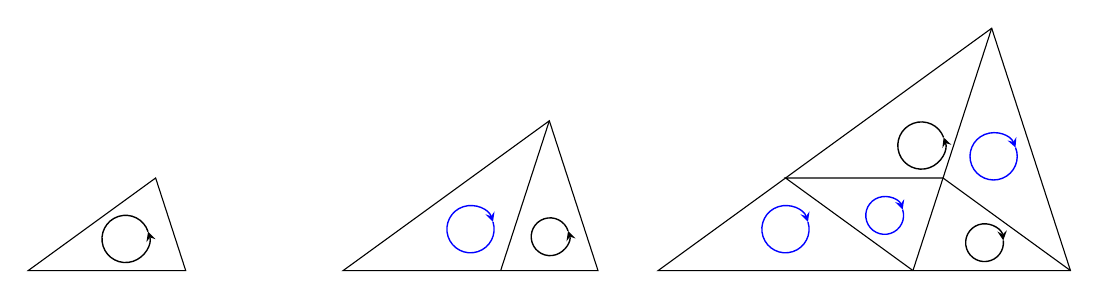
\begin{tikzpicture}[scale=2]
  \draw (0,0) -- (1,0) -- (36:1) -- cycle;
  \draw[->,>=stealth,line width=0.5] (18:0.8) arc (18:(18+360):0.15);


  \begin{scope}[xshift=2cm]
   \draw (0,0) -- (1.618,0) -- (36:1.618) -- cycle;
   \draw (1,0) -- (36:1.618);
   \draw[->,>=stealth,line width=0.5,blue] (18:1.0) arc (18:(18-360):0.15);
   \draw[->,>=stealth,line width=0.5] (10:1.45) arc ((18-360):18:0.12);
  \end{scope}

  \begin{scope}[xshift=4cm]
  \draw (0,0) -- (2.618,0) -- (36:2.618) -- cycle;
   \draw (1.618,0) -- (36:2.618);
   \draw (0:1.618)-- ++(144:1) -- ++(0:1) -- (0:2.618);
  \draw[->,>=stealth,line width=0.5,blue] (18:1.0) arc ((18+360):18:0.15);
  \draw[->,>=stealth,line width=0.5,blue] (14:1.6) arc ((18+360):18:0.12);
  \draw[->,>=stealth,line width=0.5] (25:2.0) arc (20:(20+360):0.15);
  \draw[->,>=stealth,line width=0.5,blue] (19.:2.4) arc ((22+360):22:0.15);
  \draw[->,>=stealth,line width=0.5] (5:2.2) arc ((7+360):7:0.12);

  \end{scope}
 \end{tikzpicture}
\end{center}

タイル張りを以下のようにして構成します。
初期配置は下図のような10枚のAタイプのタイル10枚から構成されます。

\begin{center}
 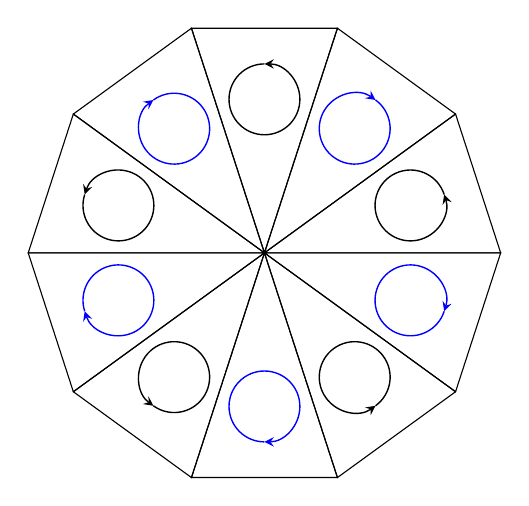
\begin{tikzpicture}[scale=3]
  \foreach \t in {0,72,...,324}{
  \draw[] (0,0)--({cos(\t)},{sin(\t)})-- ({cos(\t+36)},{sin(\t+36)}) -- cycle;
  }
  \foreach \t in {36,108,...,324}{
  \draw[] (0,0)--({cos(\t)},{sin(\t)})-- ({cos(\t+36)},{sin(\t+36)}) -- cycle;
  }
  \foreach \i in {18,90,...,324}{
  \draw[->,>=stealth,line width=0.5] (\i:0.8) arc (\i:(\i+360):0.15);
  }
  \foreach \i in {54,126,...,360}{
  \draw[->,>=stealth,line width=0.5,blue] (\i:0.8) arc ((\i+360):\i:0.15);
  }
 \end{tikzpicture}
\end{center}

ここで各タイルには向きがあり、1枚おきに向きが反転していることに
気をつけます。つまり、A型のタイルを表向き、裏向き交互に配置していると
考えます。
これに拡大細分を1回適用すると、次のようなタイル張りが出来上がります。

\begin{center}
 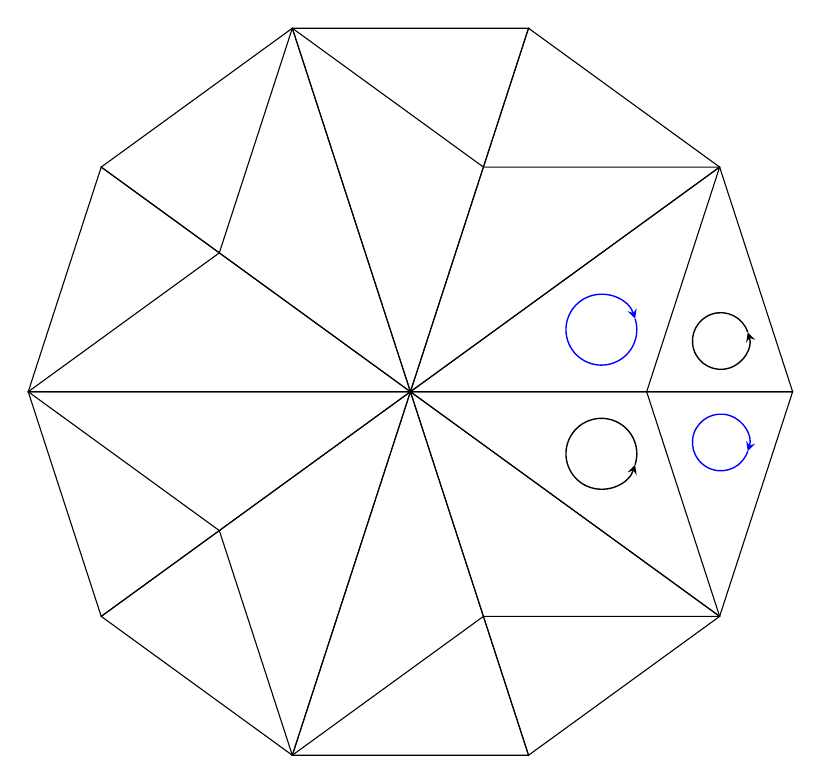
\begin{tikzpicture}[scale=3]
  \foreach \t in {0,72,...,324}{
  \draw[] (0,0)--({1.618*cos(\t)},{1.618*sin(\t)})-- ({1.618*cos(\t+36)},{1.618*sin(\t+36)}) -- cycle;
  \draw ({cos(\t)},{sin(\t)}) -- ({1.618*cos(\t+36)},{1.618*sin(\t+36)});
  }
  \foreach \t in {36,108,...,324}{
  \draw[] (0,0)--({1.618*cos(\t)},{1.618*sin(\t)})-- ({1.618*cos(\t+36)},{1.618*sin(\t+36)}) -- cycle;
  \draw ({cos(\t+36)},{sin(\t+36)}) -- ({1.618*cos(\t)},{1.618*sin(\t)});
  }
  \draw[->,>=stealth,line width=0.5,blue] (18:1) arc (18:(18-360):0.15);
  \draw[->,>=stealth,line width=0.5] (10:1.45) arc ((18-360):18:0.12);
  \draw[->,>=stealth,line width=0.5] (-18:1) arc ((-18):(-18+360):0.15);
  \draw[->,>=stealth,line width=0.5,blue] (-10:1.45) arc ((-18+360):(-18):0.12);

 \end{tikzpicture}
\end{center}

\section{プログラミング}

\subsection{言語}
本当はこういうプログラミングには向いていないのかも
しれませんが、完成品を手軽に使ってもらえるであろうから、
\verb+javascript+を使うことにしましょう。

\subsection{データ構造}
データ構造についてはどうしましょう?
タイルは多角形です。多角形は辺と頂点からなります。
頂点を$5$次元整数ベクトルで表すということまで
は決定しています。

以下は仮の提案です。
\begin{description}
 \item[頂点$v$]
       長さ$5$の配列(\verb+javascript+では\verb+list+と呼ぶ。)

 \item[頂点集合]
       頂点の配列{\verb+vertices+}、つまり配列の配列、2次元配列です。
 \item[三角形]
	    頂点集合を格納する配列\verb+vertices+のインデックスを3つ並べた
	    配列で構成します。このとき、配列の要素の並びに、
	    つまり、\underline{頂点の並べ方に意味があります}。
	    これによって三角形が表向きか、裏向きかが決まるの
	    ですが、プログラミングを進める上ではあまり
	    意識する必要はないと思います。
 \item[三角形の集合] 
	    $A$型,$B$型に分けて、三角形の集合として構成します。
\end{description}

ですから、最初状況は、下のような感じになります。


\begin{lstlisting}[caption=初期化]
let vertices = [[0,0,0,0,0],
		[1,0,0,0,0],
		[0,1,0,0,0],
		[0,0,1,0,0],
		[0,0,0,1,0],
		[0,0,0,0,1],
		[-1,0,0,0,0],
		[0,-1,0,0,0],
		[0,0,-1,0,0],
		[0,0,0,-1,0],
		[0,0,0,0,-1]
	       ];
let Atriangles = [[0,1,2],
		 [0,3,2],
		 [0,3,4],
		 [0,5,4],
		 [0,5,6],
		 [0,7,6],
		 [0,7,8],
		 [0,9,8],
		 [0,9,10],
		 [0,1,10]
		 ];
let Btriangles = [];
\end{lstlisting}

\subsection{アルゴリズム}
私達は既に頂点の$\varphi$倍(拡大)操作を実装し、
頂点$x,y$を$\varphi$倍した$\varphi{x},\varphi{y}$を
$\varphi:1$に内分した頂点の計算方法を実装しました。

これらを用いて\underline{\em 三角形の拡大細分操作}を実装していきます。
拡大操作は易しいのですが、拡大細分は少し戸惑うと思います。

A型三角形では新しい頂点が一つ発生して、B型三角形では2つ発生します。
隣接する異なる三角形で共通の新しい頂点が発生することがあり得ます。

最初は速度などはあまり気にしないで素朴に
拡大細分を実行して新しい頂点が既に\verb+vertices+に登録されているか
確認して、なければ追加\verb+push+し、そのindexを新しい三角形の
indexとして採用するというような操作で良いのかなと思います。



\end{document}